\section{Экономическая эффективность}

Для оценки экономической эффективности нужно сравнить затраты на аппаратное и
программное обеспечение, используемое в проекте. Цены на компьютерные комплектующие
взяты с сервиса агрегации цен E-katalog \cite{ref:eeekatalog}. Цены на ПО взяты с сайтов
официальных дистрибуторов ПО (или их представителей в Российской Федерации).  Для
отсутствующих в продаже компонентов взяты их современные аналоги, сравнимые по
производительности.

Так как сервер для демонстрации возможностей данного проекта собран из обычных
потребительских комплектующих, в таблице указана их стоимость. Стоит отметить, что для
сборки полноценного сервера стоит использовать специализированные серверные 
комплектующие. Их стоимость выше, однако и производительность при этом отличается в
большую сторону, что может быть полезно для дальнейшего увеличения производительности и
надежности всей системы.

Стоимость комплектующих сервера приведена в таблице \ref{tab:server_price},
комплектующих ПК — в таблице \ref{tab:pc_price}. В расчетах не учитывается стоимость
корпуса. Cтоимость Raspberry Pi 3 Model B, корпуса и блока питания в сумме принята
6000~рублей при покупке от 5~шт. \cite{ref:raspberry_price}. В расчетах не учитывается
стоимость мониторов, клавиатур и компьютерных мышек, так как они идентичны в обоих
сценариях.

Помимо аппаратного обеспечения, нужно учесть затраты на программное обеспечение для всех
клиентов. Т.к. Windows Server Essentials не требует дополнительных клиентских лицензий,
то стоимость лицензирования будет равна 17 158 руб. (для оценки взята стоимость
Microsoft Windows Server Essentials 2019, коробочная версия для академических
организаций). Для клиентских ПК взята стоимость Windows 10 OEM, равная 1 196 руб
\cite{ref:windows_price}. Для каждого клиентского ПК нужно покупать отдельную лицензию,
для системы из тонких клиентов — только серверную ОС.

Стоимость прикладного программного обеспечения варьируется в зависимости от продукта.
Например, лицензирование Solidworks для учебных заведений выполняется на всю
организацию, соответственно стоимость для одного клиента будет одинакова в обоих
сценариях.

В результате расчетов были построены графики зависимости стоимости программного и
аппаратного обеспечения от количества клиентов (см. рисунок~\ref{pic:price_chart}).
Фрагмент расчетной таблицы приведен ниже (см. таблицу~\ref{tab:price_comp}).
Экономичность расчитывается как отношение разницы в стоимости систем к стоимости системы
тонких клиентов.

Таким образом, можно сделать вывод о экономической целесообразности реализации данного
проекта. По сравнению с используемой на кафедре системой из полноценных компьютеров
(толстых клиентов), система тонких клиентов дает возможность значительно снизить затраты
при подключении требуемого количества клиентов, получая более сравнимую или более
высокую производительность рабочих мест. 

При подключении 25 клиентов, что является максимально возможным
количеством пользователей для используемой лицензии Windows Server Essentials, экономия
средств на программное и аппаратное обеспечение составляет 96\%.
Стоит отметить, что при необходимости дальнейшей модернизации, достаточно будет обновить
аппаратное обеспечение только серверной части, что также уменьшает дальнейшие затраты на
оборудование.

\begin{table}[h]
    \centering
    \caption{Оценка экономичности системы ТК}
    \label{tab:price_comp}
    \begin{tabu}to \linewidth{X[3,l]X[c,m]X[c,m]X[c,m]}
        \toprule
        Количество клиентов & 15 & 20 & 25 \\
        \midrule
        Толстые клиенты, руб & 277005 & 369340 & 461675 \\ 
Cервер и тонкие клиенты, руб & 175427 & 205427 & 235427 \\ 
\midrule
Экономия, \% & 58 & 80 & 96 \\ 

        \bottomrule
    \end{tabu}
\end{table}

\begin{figure}[h]
    \center
    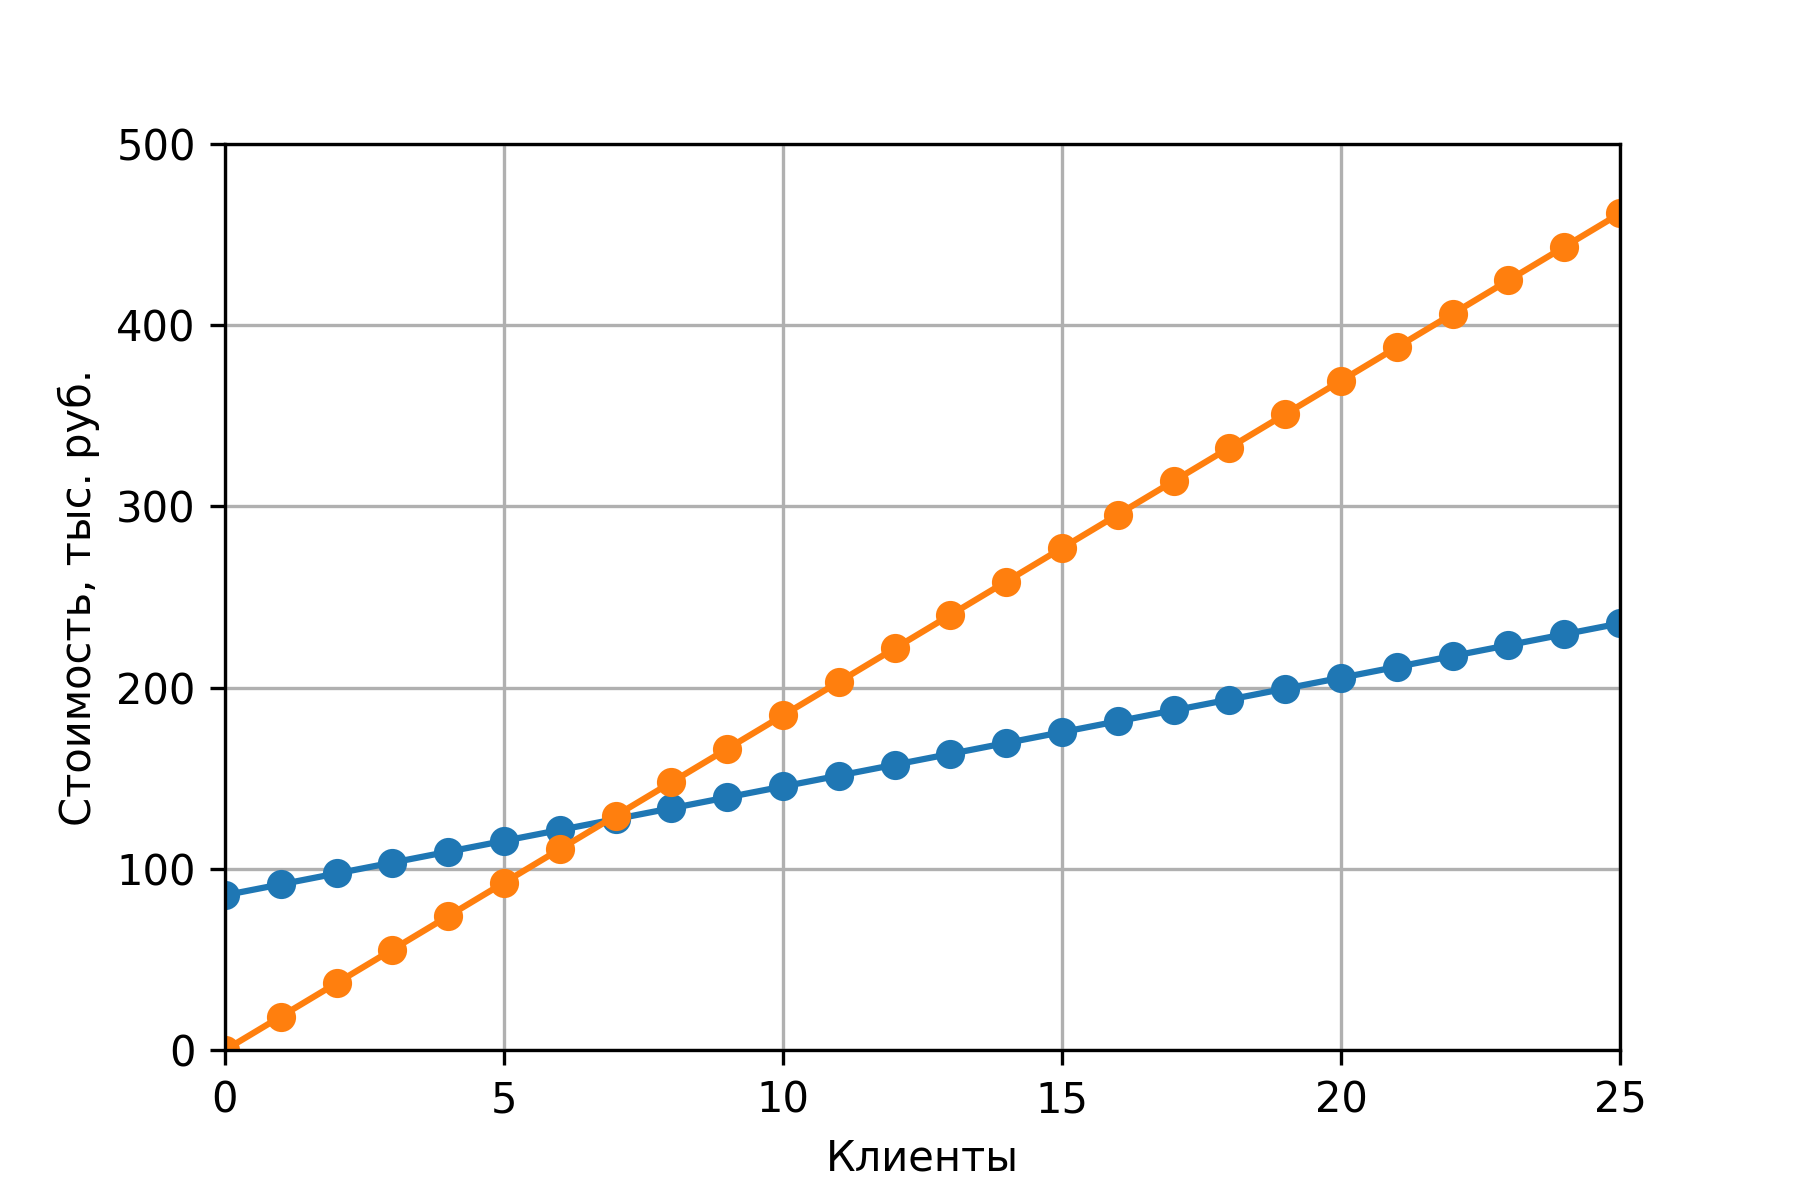
\includegraphics[width=\linewidth]{price_chart}
    \caption{Зависимость стоимости системы от количества клиентов}
    \label{pic:price_chart}
\end{figure}

\begin{table}[b]
    \centering
    \caption{Стоимость комплектующих сервера}
    \label{tab:server_price}
    \begin{tabu}to \linewidth{X[m]X[2.2,c,m]X[r,m]}
        \toprule
        Компонент & Название & Стоимость, руб \\
        \midrule
        Процессор          & AMD Ryzen 5 2600                          & 8 980  \\
        Материнская плата  & Asus PRIME X370-PRO                       & 12 590 \\
        Оперативная память & Patriot Signature 16GB PSD416G26662, 2 шт & 9 998   \\
        Видеокарта         & Sapphire Radeon RX 580 PULSE 8GB          & 16 138  \\
        Накопитель         & Samsung 860 EVO 500 ГБ                    & 6 060  \\
        Блок питания       & Be quiet! Straight Power 11 850 Вт        & 14 503 \\
        Лицензия           & Windows Server Essentials 2019            & 17 158 \\
        \midrule
        Итог & & 85 427 \\
        \bottomrule
    \end{tabu}
\end{table}

\begin{table}[t]
    \centering
    \caption{Стоимость комплектующих рабочего ПК}
    \label{tab:pc_price}
    \begin{tabu}to \linewidth{X[m]X[2.2,c,m]X[r,m]}
        \toprule
        Компонент & Название & Стоимость, руб \\
        \midrule
        Процессор          & Intel Core i3-9100F            & 5 721 \\
        Материнская плата  & Asus PRIME B360M-A             & 5 893 \\
        Оперативная память & Crucial Value 4Gb CT4G4DFS824A & 1 331 \\
        Видеокарта         & Интегрированная в процессор    & —     \\
        Накопитель         & Kingston A400 120 ГБ           & 1 960 \\
        Блок питания       & FSP ATX-500PNR                 & 2 366 \\
        Лицензия           & Windows 10 OEM                 & 1 196 \\
        \midrule
        Итог & & 18 467 \\
        \bottomrule
    \end{tabu}
\end{table}

\fixme{Анализ на устойчивость}
